\begin{enumerate}
\item The dimensions of a solid iron cuboid are $4.4$ m $\times$ $2.6$ m $\times$ $1.0$ m. It is melted and recast into a hollow cylindrical pipe of $30$ cm inner radius and thickness $5$ cm. Find the length of the pipe. 
\item From a solid right circular cylinder of height $2·4$ cm and radius $0·7$ cm, a right circular cone of same height and same radius is cut out. Find the total surface area of the remaining solid.
\item Three semicircles each of diameter $3$ cm, a circle of diameter $4.5$ cm and a semicircle of radius $4.5$ are drawn in the given figure. Find the area of the shaded region.
\begin{figure}[H]
\centering
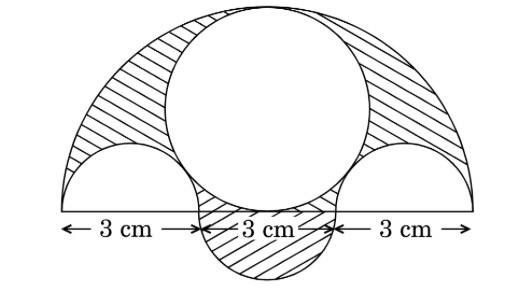
\includegraphics[width = 0.6\columnwidth]{figs/geo1.jpg}  
\end{figure}
\item In the given figure, two concentric circles with centre $O$ have radii $21$ cm and $42$ cm. If $\angle AOB = 60\degree$, find the area of the shaded region.
\hfill $\sbrak{Use \pi = \frac{22}{7}}$
\begin{figure}[H]
\centering
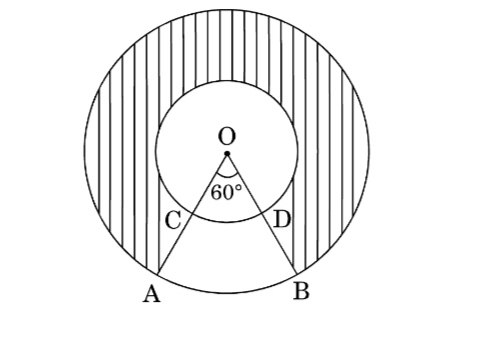
\includegraphics[width=0.6\columnwidth]{figs/geo2.jpg}
 \end{figure}
\item In the given figure, $\triangle$ $ABC$ is a right-angled triangle in which $\angle{A}$ = 90$\degree$. Semicircles are drawn on $AB$, $AC$ and $BC$ as diameters. Find the area of the shaded region.
\begin{figure}[H]
\centering
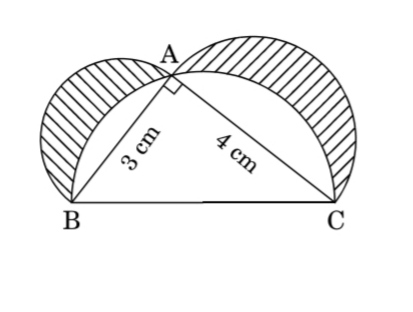
\includegraphics[width=0.8 \columnwidth]{figs/geo3.jpg}
\end{figure}
\item In the figure $O$ is the centre of the circle with $AC = 24$ cm, $AB = 7$ cm, and $\angle BOD = 90\degree$. Find the area of the shaded region.
\begin{figure}[H]
\centering
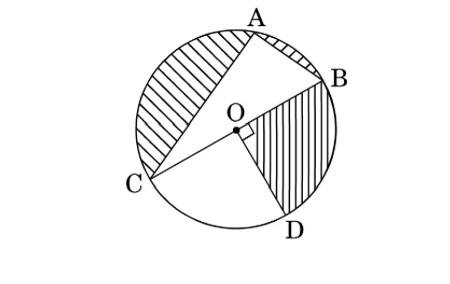
\includegraphics[width = 0.6\columnwidth]{figs/geo4.jpg}
\end{figure}
\item In the given figure, $ABCD$ is a rectangle of dimensions $21$ cm x $14$ cm. A semicircle is drawn with $BC$ as diameter. Find the area and the perimeter of the shaded region in the figure.
\begin{figure}[H]
\centering
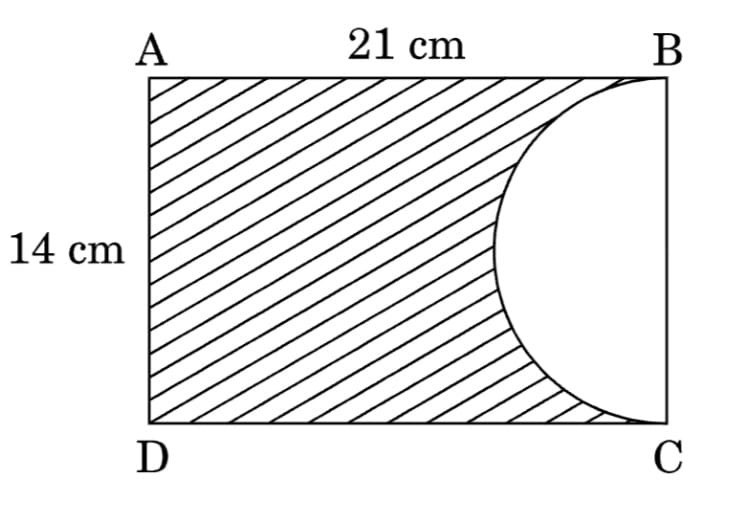
\includegraphics[width = 0.6\columnwidth]{figs/geo5.jpg}
\end{figure}
\item A toy is in the form of a cone of radius $3.5$ cm mounted on a hemisphere of same radius on its circular face. The total height of the toy is 15.5 cm. Find the total surface area of the toy.
\begin{figure}[H]
\centering
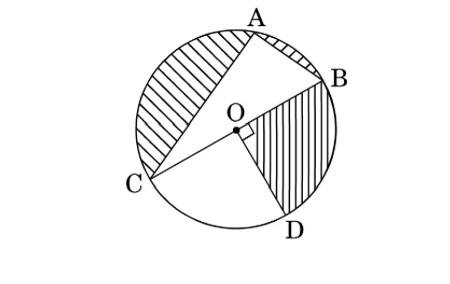
\includegraphics[width=0.5\linewidth]{figs/geo6.jpg}
\label{fig:enter-label}
\end{figure}
\item In a rain-water harvesting system, the rain-water form a roof of $22$ m $\times$ $20$ m drains into a cylindrical tank having diameter of base $2$ m and height $3.5$ m. If the tank is full, find the rainfall in cm. Write your views on water conservation.
\item The slant height of a frustum of a cone is $4$ cm and the perimeters of its circular ends are $18$ cm and $6$ cm. Find the curved surface area of the frustum.
\end{enumerate}
